%----------------------------------------------------------------------------------------
%	PACKAGES AND OTHER DOCUMENT CONFIGURATIONS
%----------------------------------------------------------------------------------------

\documentclass[11pt]{article}

\usepackage[utf8]{inputenc}
\usepackage[T1]{fontenc}
\usepackage[english, brazilian]{babel}

\usepackage{amsmath}
\usepackage{amsfonts}
\usepackage{amssymb}

\usepackage{appendix}
\usepackage[nottoc,numbib]{tocbibind}

\usepackage{graphicx}
\usepackage{kpfonts}
\usepackage{booktabs}
\usepackage{listings}
\usepackage{color}

\usepackage{pdfpages}

\lstset{
  language=Python,
  showstringspaces=false,
  formfeed=newpage,
  tabsize=4,
  commentstyle=\itshape,
  basicstyle=\ttfamily,
  morekeywords={models, lambda, forms}
}

\renewcommand{\appendixtocname}{Anexo}
\renewcommand{\appendixpagename}{Anexo}

\begin{document}

\begin{titlepage}

\newcommand{\HRule}{\rule{\linewidth}{0.5mm}} % Defines a new command for the horizontal lines, change thickness here

\center % Center everything on the page

%----------------------------------------------------------------------------------------
%	LOGO SECTION
%----------------------------------------------------------------------------------------


\includegraphics[scale=1.2]{ufulogo4}\\[1cm] % Include a department/university logo - this will require the graphicx package
 
%----------------------------------------------------------------------------------------

%----------------------------------------------------------------------------------------
%	HEADING SECTIONS
%----------------------------------------------------------------------------------------

%\textsc{\LARGE Universidade Federal de Uberlândia}\\[0.5cm] % Name of your university/college
\textsc{\Large Faculdade de Engenharia Elétrica}\\[0.6cm] % Major heading such as course name
{\large 3º trabalho de Inteligência Artificial}\\[0.5cm] % Minor heading such as course title

%----------------------------------------------------------------------------------------
%	TITLE SECTION
%----------------------------------------------------------------------------------------

\HRule \\[0.4cm]
{ \huge \bfseries Regra de Hebb para treinamento de redes neurais artificiais}\\[0.4cm] % Title of your document
\HRule \\[1.5cm]
 
%----------------------------------------------------------------------------------------
%	AUTHOR SECTION
%----------------------------------------------------------------------------------------

\begin{minipage}{0.4\textwidth}
\begin{flushleft} \large
\emph{Aluno}\\
Roní G.\ \textsc{Gonçalves}\\% Your name
\end{flushleft}
\end{minipage}
~
\begin{minipage}{0.4\textwidth}
\begin{flushright} \large
\emph{Professor} \\
Keiji \textsc{Yamanaka}\\ % Supervisor's Name
\end{flushright}
\end{minipage}\\[0.1cm]
~
\begin{minipage}{0.85\textwidth}
\begin{flushleft} \large
10921EEL026 % Your name
\end{flushleft}
\end{minipage}\\[3cm]
~
% If you don't want a supervisor, uncomment the two lines below and remove the section above
%\Large \emph{Author:}\\
%John \textsc{Smith}\\[3cm] % Your name

%----------------------------------------------------------------------------------------
%	DATE SECTION
%----------------------------------------------------------------------------------------

{\large Uberlândia, \today}\\[1cm] % Date, change the \today to a set date if you want to be precise


\vfill % Fill the rest of the page with whitespace

\end{titlepage}

\setcounter{page}{2}

\newpage

\begin{abstract}
Um programa usando o método de treinamento de neurônios artificias pela regra de Hebb é desenvolvido para implementar todas as portas lógicas com duas entradas. O programa foi criado com a combinação de Python, GTK+ 3, GtkBuilder e Glade.

\emph{Palavras-chave}: inteligência artificial, neurônios artificiais, regra de Hebb, portas lógicas, Python, GTK+ 3.
\end{abstract}

\begin{otherlanguage}{english}
\begin{abstract}
An application that implements all the two-entries logic gates was developped using the Hebb's rule to train the artificial neural network.
It was created using Python, GTK+ 3, GtkBuilder and Glade. 

\emph{Keywords}: artificial intelligence, artificial neurons, Hebb's rule, logic gates, Python, GTK+ 3.
\end{abstract}
\end{otherlanguage}

\newpage
\tableofcontents
\newpage

\section{Introdução}

Por meio da combinação da linguagem de programação Python, do editor gráfico de interfaces Glade, da biblioteca gráfica GTK+ 3 e do GtkBuilder\footnote{Módulo responsável por fazer a ligação entre a interface gráfica feita no Glade em formato XML e o código desenvolvido em Python.} desenvolvi um programa com interface gráfica que ilustra o uso da regra de Hebb para treinar uma rede neural artificial, que é capaz de recriar o comportamento de qualquer porta lógica de duas entradas.

Primeiramente, apresento a regra de Hebb para o treinamento da rede neural artificial. Logo após, cada elemento necessário à criação do programa é brevemente explicado.

Ao final, algumas conclusões são tomadas a partir dos resultados. Algumas perspectivas de melhorias no programa são apresentadas.

Todos os códigos usados no programa se encontram presentes no anexo deste trabalho.    

\section{A regra de Hebb}

A regra de Hebb\footnote{Também conhecida como teoria hebbiana, nome em homenagem ao pesquisador Donald Hebb.} foi uma das primeiras propostas de treinamento de redes neurais artificiais.

Tal regra pode ser enunciada da seguinte forma: \emph{se dois neurônios interligados estiverem ativados ou desativados simultaneamente, o peso desta conexão deve ser aumentado}.

\subsection{Algoritmo para duas entradas e uma saída}\label{sec:algoritmo}

Considerando que as entradas e as saídas só possam assumir dois valores, o seguinte algoritmo se aplica para a determinação dos pesos das sinapses dos neurônios artificiais:

\begin{enumerate}
\item Inicializar os pesos iguais a zero: $w_1 \leftarrow 0$; $w_2 = 0$ e $b \leftarrow 0$.

\item Para cada par entradas-saída ([$e_1$, $e_2$], t), fazer: $x_1 \leftarrow e_1$; $x_2 \leftarrow e_2$; $y \leftarrow t$.

\item Definir: $\Delta w_1 \leftarrow x_1 y$, $\Delta w_2 \leftarrow x_2 y$.

\item Atualizar os pesos: $w_1 \leftarrow w_1 + \Delta w_1$, $w_2 \leftarrow w_2 + \Delta w_2$ e $b \leftarrow b + y$.
\end{enumerate}

\section{Programação}

O programa \emph{gamb.IA.rra} foi escrito em Python (www.python.org), que segundo o próprio site: \emph{ é uma linguagem interpretada, interativa, orientada a objetos. Ela incorpora módulos, exceções, tipagem dinâmica, estruturas de dados altamente dinâmicas e classes. O Python combina grande poder com sintaxe clara. Ele possui interfaces para inúmeras chamadas de sistemas e bibliotecas, assim como para inúmeros sistemas operacionais e ainda é extensível em C e C++} [\ldots]

\subsection{Esboço da interface gráfica}

Na figura \ref{fig:esboco} é mostrada como a janela principal do programa deveria ser. O esboço foi feito no programa Pencil (http://pencil.evolus.vn/)

\begin{figure}[h]
\centering
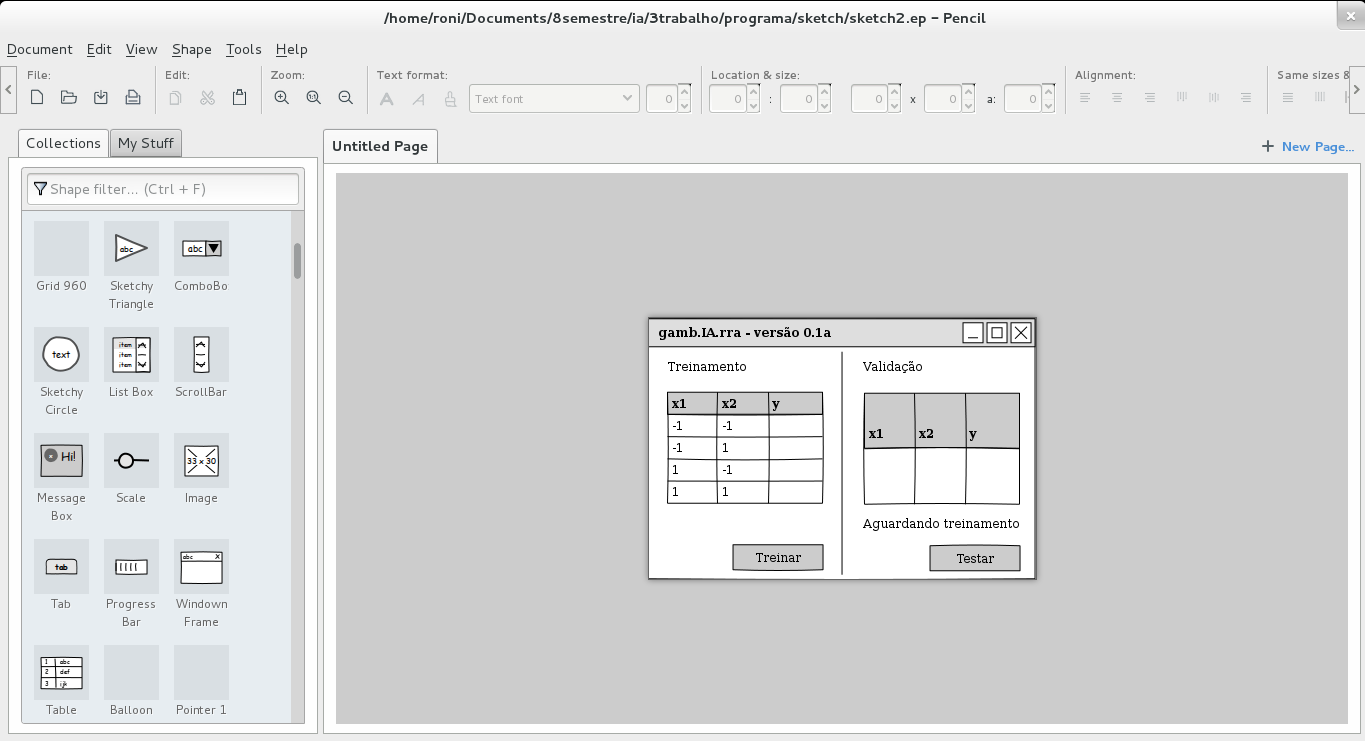
\includegraphics[scale=0.30]{figuras/pencil}
\caption{Janela principal do programa Pencil.}
\end{figure}

\begin{figure}[h]
\centering
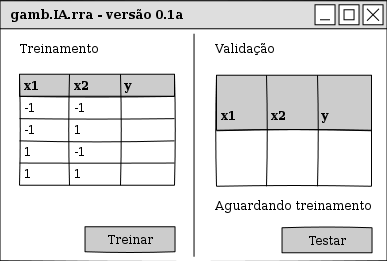
\includegraphics[scale=0.5]{../programa/sketch/figura1}
\caption{Esboço da interface gráfica do programa gamb.IA.rra.}\label{fig:esboco}
\end{figure}

No lado esquerdo da janela principal, existe a área \emph{Treinamento} onde o usuário pode inserir os valores da saída que ele quiser: isso caracteriza uma porta lógica. Variando os valores de saída, o usuário pode ter portas lógicas \emph{e}, \emph{ou}, \emph{não e} \ldots

Após inserir os quatro valores desejados, o usuário deve pressionar o botão \emph{Treinar}, dessa forma o algoritmo apresentado na seção \ref{sec:algoritmo} é usado e os pesos são determinados. Quando o treinamento termina, o rótulo \emph{Aguardando treinamento} presente na área \emph{Validação} à esquerda da janela principal indica que está pronta passando a exibir o texto \emph{Treinamento completo}.

Uma vez feito o treinamento, o usuário pode testar se os pesos calculados funcionam realmente para quaisquer entradas $x_1$ e $x_2$ que ele digite na área \emph{Validação}.

\subsection{Interface gráfica em XML}

O programa Glade (glade.gnome.org) foi usado para desenhar a interface gráfica proposta na figura \ref{fig:esboco}. A janela principal do Glade pode ser vista logo a seguir.

\begin{figure}[h]
\centering
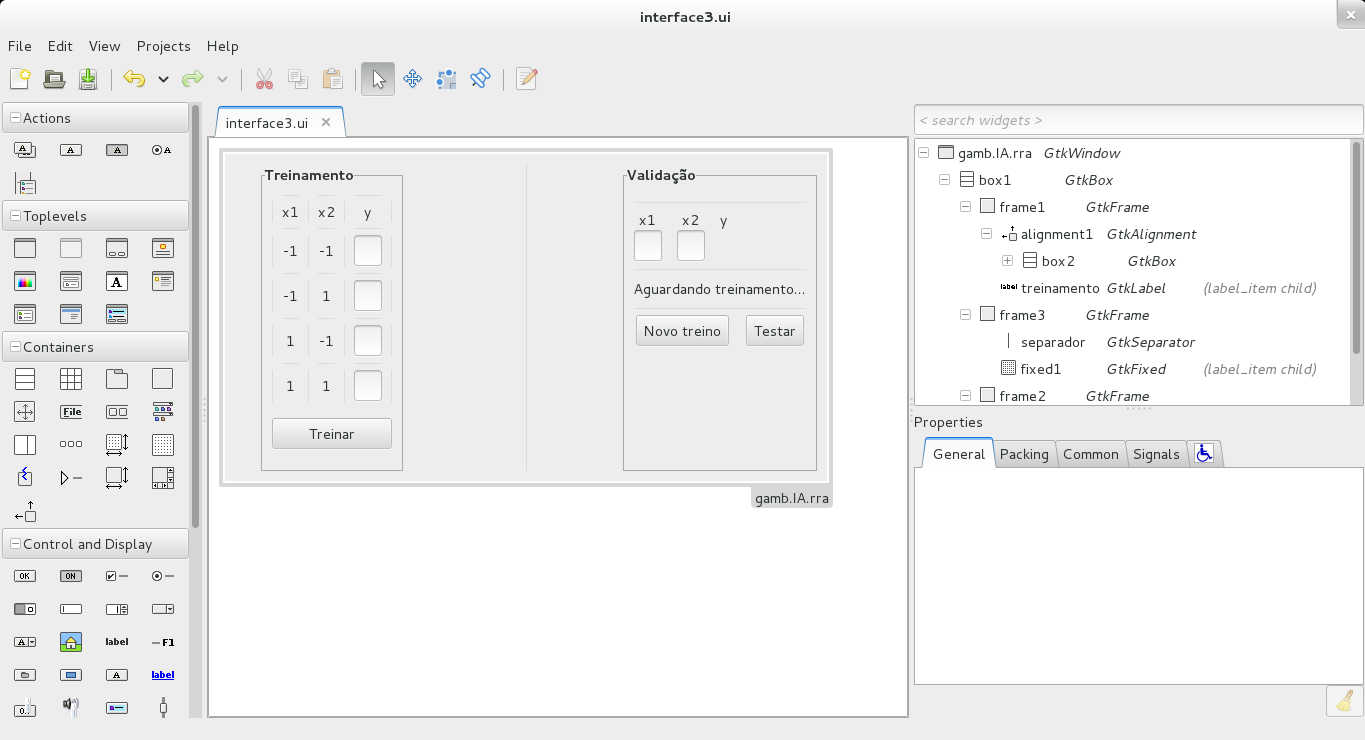
\includegraphics[scale=0.3]{figuras/glade}
\caption{Janela principal do programa Glade usado para criar a interface gráfica do programa gamb.IA.rra.}\label{fig:glade}
\end{figure}

\subsection{Construtor GTK+}

O GtkBuilder é o responsável por pegar o arquivo XML criado no Glade e transformá-lo em objetos de interface gráfica do GTK+. Além disso, ele associa os eventos ocorridos ao usar o programa como, por exemplo, clicar um botão aos seus objetos denominados \emph{handlers}.


\begin{lstlisting}[frame=single]
#Construindo interface e associando sinais a callbacks
builder = Gtk.Builder()
builder.add_from_file('../ui/interface3.ui')
builder.connect_signals(handlers)
\end{lstlisting}
%\inputlistings{}

\subsection{Programa feito: gamb.IA.rra}

Com o uso de todas as ferramentas citadas acima, o resultado final pode ser conferido na figura \ref{fig:gamb1}

\begin{figure}[h]
\begin{center}
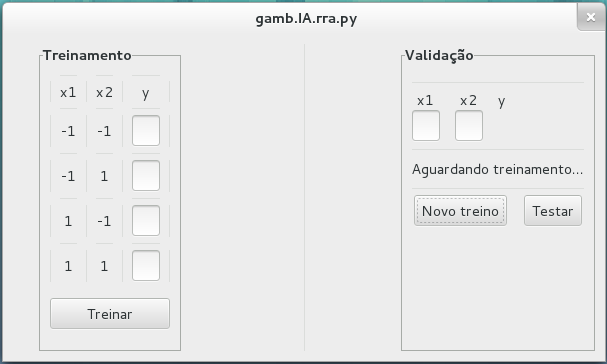
\includegraphics[scale=0.6]{figuras/gamb1}
\caption{Janela principal e única do programa feito.}\label{fig:gamb1}
\end{center}
\end{figure}

Um caso de uso é mostrado na seqüência: o usuário digita os valores de saída que ele quer (figura \ref{fig:gamb2}), clica no botão \emph{Treinar} (figura \ref{fig:gamb3}), testa se o programa aprendeu o comportamento da porta lógica com o par de entrada igual a 1 (figura \ref{fig:gamb4}) clicando no botão \emph{Testar} (figura \ref{fig:gamb5}).

\begin{figure}[p]
\begin{center}
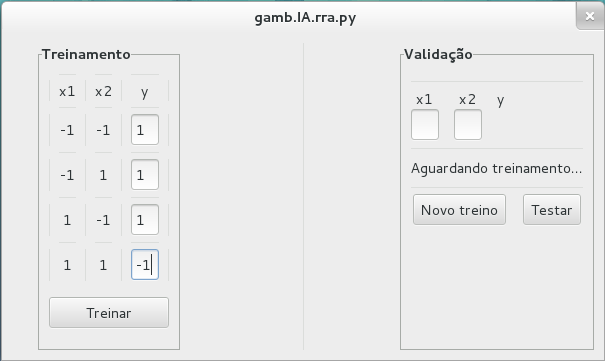
\includegraphics[scale=0.6]{figuras/gamb2}
\caption{O usuário entra com os dados desejados para criar uma tabela-verdade e, conseqüentemente, uma porta lógica de duas entradas para realizar o treinamento da rede neural.}\label{fig:gamb2}
\end{center}
\end{figure}

\begin{figure}[p]
\begin{center}
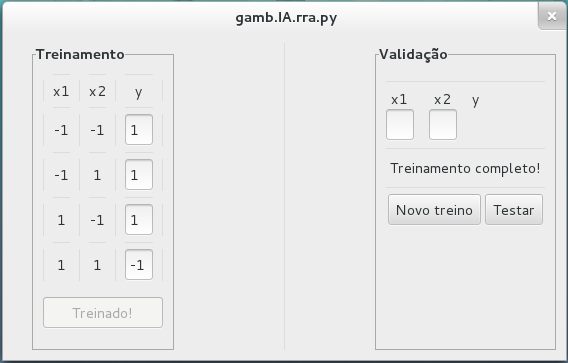
\includegraphics[scale=0.6]{figuras/gamb3}
\caption{Após clicar no botão \emph{Treinar}, os pesos são determinados pela regra de Hebb e o usuário pode, então, testar se a rede neural aprendeu corretamente a tabela verdade.}\label{fig:gamb3}
\end{center}
\end{figure}

\begin{figure}[p]
\begin{center}
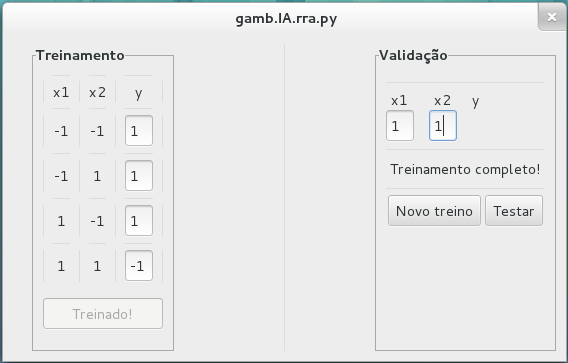
\includegraphics[scale=0.6]{figuras/gamb4}
\caption{O usuário entra com os dados para realizar o teste e conferir se o resultado é igual ao esperado.}\label{fig:gamb4}
\end{center}
\end{figure}

\begin{figure}[p]
\begin{center}
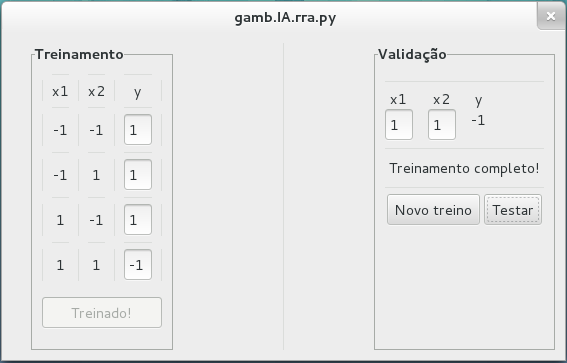
\includegraphics[scale=0.6]{figuras/gamb5}
\caption{O usuário confirma que para o par de entradas (1,1) gera a saída esperada -1.}\label{fig:gamb5}
\end{center}
\end{figure}

\section{Conclusões}

A regra de Hebb constitui-se numa primeira tentativa de determinar os pesos das ligações sinápticas de neurônios artificiais. Em vez de usar o método da tentativa e erro, pode-se aplicá-la com razoável sucesso para implementar portas lógicas.

Há um porém: somente problemas linearmente separáveis podem ser resolvidos com este método. De tal forma que os pesos obtidos para as portas lógicas \emph{ou exclusivo} e \emph{não ou exclusivo} não são válidos.

A interface gráfica criada ajuda no entendimento e no uso dos neurônios artificiais. No entanto, muitas melhorias ainda podem e serão feitas.

\newpage
\begin{thebibliography}{3}

\bibitem{Yamanaka}
  Keiji Yamanaka,
  \emph{Notas de aula da disciplina Inteligência Artificial}.
  Faculdade de Engenharia Elétria, Universidade Federal de Uberlândia, 2014.

\bibitem{Python}
  Kenneth Lambert,
  \emph{Fundamentals of Python: From first programs through data structures}.
  Cengage Learning, 2010.

\bibitem{GTK}
  Sebastian Pölsterl,
  \emph{The Python GTK+ 3 tutorial}. Versão 3.4, 24 de abril de 2014.

\end{thebibliography}

\newpage
\appendix
\appendixpage
\addappheadtotoc

\lstinputlisting[caption=\lstname, frame=single]{../programa/code/gamb.IA.rra.py}

%\lstinputlisting[caption=\lstname]{../programa/ui/interface3.ui}

\end{document}